\documentclass{article}

\usepackage{amsmath,amsthm,amsfonts,amssymb,bm}
\addtolength{\textheight}{5.0cm}
\addtolength{\voffset}{-3.5cm}
\addtolength{\hoffset}{-2.5cm}
\addtolength{\textwidth}{4.0cm}

%\allowdisplaybreaks

%\usepackage{subeqnarray}
\usepackage{mathrsfs}
\usepackage{color}
%\usepackage{url}
\usepackage{ulem}
\usepackage{indentfirst}
%\usepackage{textcomp}
%\usepackage{graphics}
%\usepackage{graphicx}
%\usepackage[hang,small,bf]{caption}
%\setlength{\captionmargin}{50pt}


%\usepackage{tikz}
%\usetikzlibrary{mindmap,trees}
\usepackage{graphicx}
%\usepackage[hang,small,bf]{caption}
%\setlength{\captionmargin}{50pt}

\graphicspath{{Figures/}{Figures/CPL/}}

\begin{document}
\title{Power Spctrum \& Its Evolution}
\author{MA Lei}
%\maketitle



\section{Growth Factor}

\begin{quote}
\bf {Scalar quantities are expanded by scalar harmonic functions Y and its first and second derivitives.}
\end{quote}

In synchronous gauge, sticking to Kodama \& Sasaki's notations, the perturbed metric is
\begin{eqnarray*}
g_{00}&=&-a^2(1+2AY) \\
g_{0j}&=&-a^2BY \\
g_{ij}&=&a^2(\gamma_{ij}+2H_LY\gamma_{ij}+2HTY_{ij}).
\end{eqnarray*}



Follow this form, Kodama et al get the basic equations for matter ($w=0$, $c_s^2=0$ for late era), which are\footnote{H. Kodama \& M. Sasaki, Progress of Theoretical Physics Supplement No. 78, 1984. Page 42,43, equation (1.18), equation (1.24), equation (1.26)}



\begin{eqnarray}
\delta'=-kv+\frac 1 2 h_L'  \label{delta1} \\
v'+\frac{a'}{a}=0 \label{v1} \\
h_L''+\frac{a'}{a}h_L'=-\chi^2\rho a^2 \delta \label{hL1}
\end{eqnarray}
where $\chi^2=8\pi G$, $h_L=2\times 3H_L$ and prime stands for $\mathrm d/\mathrm d\tau$.

Take the second derivative of eqn \ref{delta1} and multiply by $a'/a$ then subtract \ref{delta1}. Finally we get 
\begin{equation}
\delta''+H\delta'-4\pi G \rho a^2 \delta=0      .
\end{equation}

\subsection{sCDM \& LCDM}

This is a second ODE, making use of the particular solution $H$, we get the general solution,
\begin{equation}
\delta=\text{Const1}H(a)+\text{Const2}H(a)\int_0^a(\frac{1}{\tilde a H(\tilde a)})^3\mathrm d\tilde a      .
\end{equation}

We should drop the first term because this is a decaying mode.


Assume we have a initial condition, $\delta_i\equiv\delta_{i}(a_{i})$,
\begin{eqnarray}
&& \text{Const2}*H\int_0^{a_i}\frac{1}{(\tilde a H(\tilde a))^3}\mathrm d\tilde a \\
\Rightarrow && \text{Const2}=\frac{\delta_i}{H(a_i)}\frac{1}{\int_0^{a_i}1/(\tilde a H(\tilde a))^3\mathrm d\tilde a}    .
\end{eqnarray}

To simplify this solution, define
\begin{equation}
D_+(a)=\frac 52 \Omega_{m0} H(a)H_0^2\int_0^a\frac{1}{(\tilde a H(\tilde a))^3}\mathrm d\tilde a.\label{eq:GrowthFactorLCDM}
\end{equation}

Hence we have
\begin{equation}
\text{Const2}=\delta_i\frac{\frac 52\Omega_{m0}H_0^2}{D_+(a_i)}.
\end{equation}

The final expression for matter density contrast is
\begin{equation}
\delta(a)=\delta_i\frac{1}{D_+(a_i)}D_+(a).
\end{equation}

{\color{red}

This calculation is only for sCDM and LCDM. One approximation for growth factor for other DE models is 
\begin{equation}
D_+(a)\sim a\cdot \mathrm{exp}[\int_a^1 \frac{\mathrm da}{a}(1-\Omega_m^\alpha)]
\end{equation}

while 
\begin{equation}
\alpha=\frac{3}{5-\frac{w}{1-w}}+\frac{3}{125}\frac{(1-w)(1-3w/2)}{(1-6w/5)^3}(1-\Omega)+\mathcal O((1-\Omega)^2)  .
\end{equation}


There are other papers on this issue:
9804015 \& 0703779 .


}









\subsection{Other Models}


{\color{blue}

For non-interacting models, the basic equations used in calculating the the perturbation equation of matter/dark matter in {\bf Synchronous Gauge} are:

\begin{eqnarray}
v' + \frac{a'}{a}v &=& 0 \\
\delta' = [-k^2 + \frac 3 2 \chi^2\rho a^2]\frac{v}{k} + ()
\end{eqnarray}


For other {\bf non-interacting} models, the function for growth factor is
\begin{equation}
\ddot\delta+2\frac{\dot a}{a}\dot\delta-\frac1 2\chi^2\rho \delta=0 \label{MatterPerturbation}
\end{equation}
in which both $\delta$ and $\rho$ are for matter.

Equation \ref{MatterPerturbation} can be written as the derivative of $a$,
\begin{eqnarray}
&& \delta''+(\frac 3 a + \frac {H'}{H})\delta'-\frac 12 \chi^2 \rho\delta\frac{1}{{\dot a}^2}=0
\end{eqnarray}

From the Freedmann equations $H^2=\frac{1}{3}\chi^2(\rho+\rho_d)$ and $2\frac{\ddot a}{a}+H^2=-\chi^2 w\rho_d$, we can find an expression for $\rho$ (matter only)
\begin{equation}
\rho=\frac{3H^2}{\chi^2}+\frac{1}{\chi^2} \frac{1}{w} (2a H H'+3H^2)
\end{equation}

Finally, in term of $a$,
\begin{eqnarray}
\delta''+(\frac{3}{a}+\frac{H'}{H})\delta'=[\frac{3}{2}(1+\frac{1}{w})\frac{1}{a^2}+\frac{1}{w}\frac{H'}{aH}]\delta
\end{eqnarray}

Assuming $\delta=\delta_i \frac{D_+(a)}{D_+(a_i)}$, we can get the evolution equaiton for growth factor,
\begin{equation}
D_+''+(\frac{3}{a}+\frac{H'}{H})D_+'=[\frac{3}{2}(1+\frac{1}{w})\frac{1}{a^2}+\frac{1}{w}\frac{H'}{aH}]D_+   \label{GrowthFactorEvolution}
\end{equation}

Will this equaiton have an analytical solution? If not we have to solve it numerically.

Physically, the solution for $D_+(a)$ for different models should be the same at early time or equivalently at small $a$. Thus we can define $r=\frac{D_+(a)}{a}$, and equation (\ref{GrowthFactorEvolution}) will become,
\begin{equation}
r''+(\frac{5}{a}+\frac{H'}{H})r'+\frac{1}{a}(\frac{3}{2a}+\frac{H'}{H})(1-\frac{1}{w})r=0
\end{equation}

There is an approximation of equation \ref{GrowthFactorEvolution} is

\begin{equation}
D''(a)+\frac{3}{2a}(1+\mathcal {H}^{-2}\Omega_{DE0})D'(a)-\frac{3}{2a^2}\mathcal H^{-2}a^{-3}D(a)=0\label{GrowthFactorEvo2}
\end{equation}

Equation \ref{GrowthFactorEvo2} and equation \ref{GrowthFactorEvolution} are identical at late times ($z$ at about a few hundred).



\begin{quote}
\begin{quote}
\begin{quote}
Useful relations:
\begin{equation}
\Omega=\frac{8\pi G\rho}{3H^2}
\end{equation}

\end{quote}
\end{quote}
\end{quote}


%%%%%%%%%%%%%%%%%%% End of Other Models%%%%%%%%%%%%%%%%%%%%%

}  







{\color{blue}

\subsection{CPL}




Figure \ref{fig:PowerSpectrum_CPL_SynchronousGauge_2012-02-19} CPL results: $w2$: $w20=-1$, $w2a=0.1$; $w3$: $w30=-1$, $w3a=-0.1$; $w4$: $w40=-0.92$, $w4a=0.35$; $w5$: $w50=-0.9$, $w5a=0.1$.

\sout{It is strange that the model with EoS $w3$ is barely distingushed from LCDM model.} All CPL Models start to deviate from LCDM model at $k\sim 0.03 h MPc^{-1}$, which is very large and perturbations come to horizon very early. Finally they have different peaks with LCDM model. For those models with EoS $w<-1$ when $a<1$, the power sepctrum go down faster than LCDM when $k$ becomes smaller and for those models with EoS $w>-1$ when $a<1$ the power spectrum go down slower than LCDM. These properties are also revealed in figure \ref{fig:QFactor_CPL_SynchronousGauge_2012-02-19}.

The truth that CPL power spectrum begin to deviate from LCDM at very early time can be seen from the evolution of growth factors, i.e., figure \ref{fig:Growth2_CPL_SynchronousGauge_2012-02-19}


Figure \ref{fig:Growth_CPL_SynchronousGauge_2012-02-19} is the growth of different models.

Figure \ref{fig:QFactor_CPL_SynchronousGauge_2012-02-19} is the Q factors, which are defined as $Q=(\frac{\delta_L}{\delta_X})^2$.

Figure \ref{fig:EoS_CPL_Sync_2012-02-19} gives the EoS.
\begin{itemize}
\item[-]
$w2$ remains larger than $-1$ before $a=1$ and has a large negative slope.
\item[-]
$w3$ remains smaller than $-1$ before $a=-1$ and has a small positive slope.
\item[-]
$w4$ remains larger than $-1$ before $a=1$ and has a slope smaller than $w2$'s.
\item[-]
$w5$ remains larger than $-1$ before $a=1$ and has a slope smaller than $w4$'s but still negative.
\end{itemize}



\begin{figure}[!htbp]
\centering
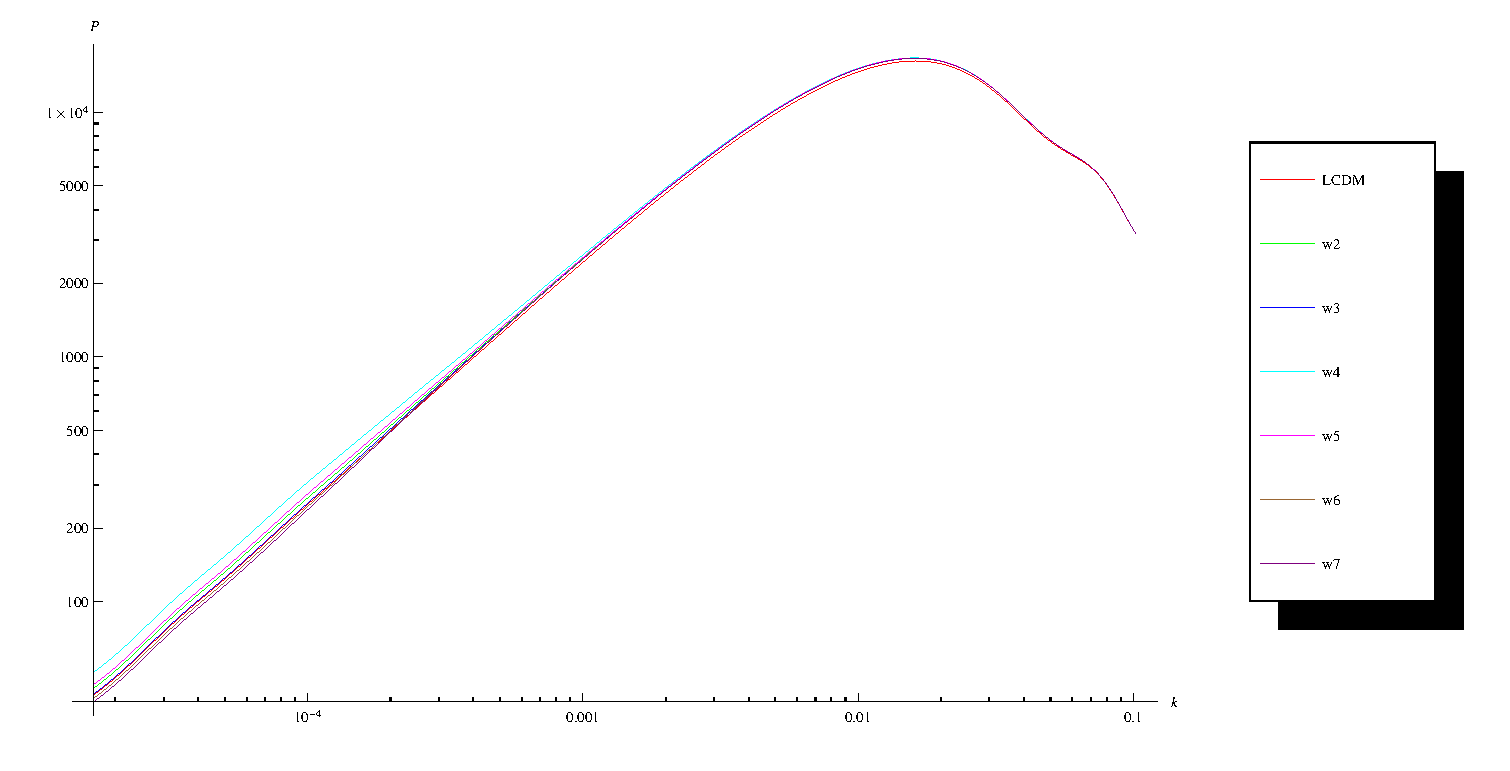
\includegraphics[width=400pt]{CPL_Sync_2012-02-20_PowerSpectrum.eps}
\caption{CPL parameteriztion. $w2$: $w20=-1$, $w2a=0.1$; $w3$: $w30=-1$, $w3a=-0.1$; $w4$: $w40=-0.92$, $w4a=0.35$; $w5$: $w50=-0.9$, $w5a=0.1$.}\label{fig:PowerSpectrum_CPL_SynchronousGauge_2012-02-19}
\end{figure}


\begin{figure}[!htbp]
\centering
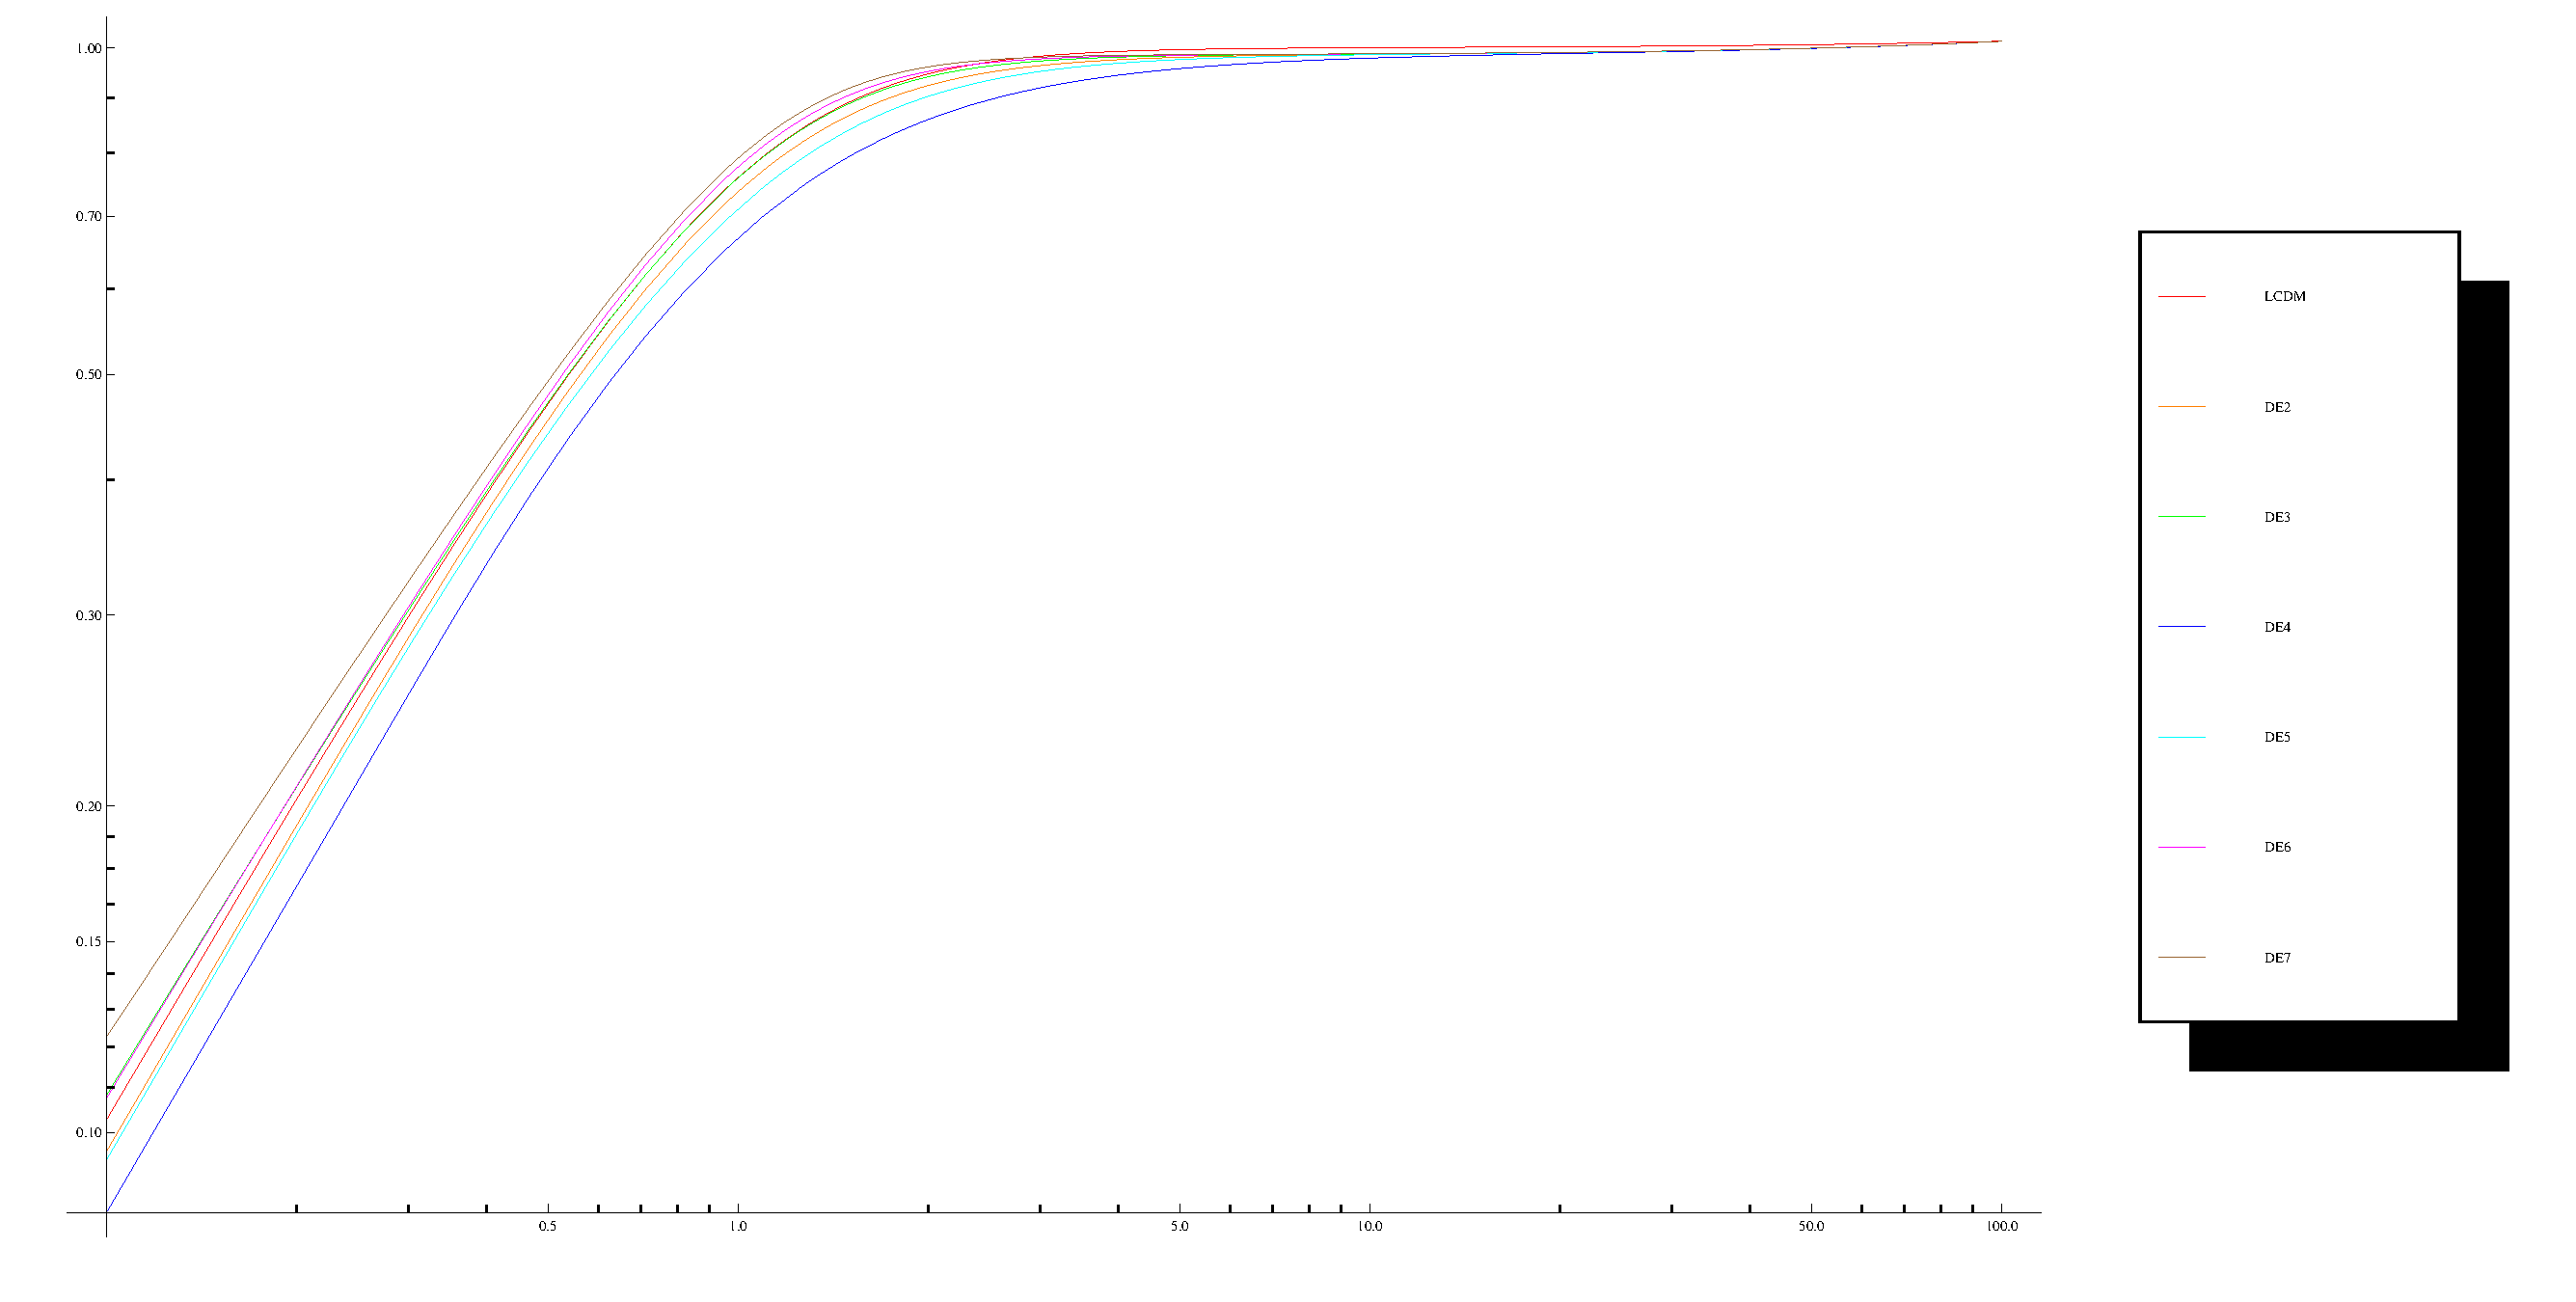
\includegraphics[width=400pt]{CPL_Sync_2012-02-20_Growth.eps}
\caption{CPL parameteriztion. $w2$: $w20=-1$, $w2a=0.1$; $w3$: $w30=-1$, $w3a=-0.1$; $w4$: $w40=-0.92$, $w4a=0.35$; $w5$: $w50=-0.9$, $w5a=0.1$.}\label{fig:Growth_CPL_SynchronousGauge_2012-02-19}
\end{figure}


\begin{figure}[!htbp]
\centering
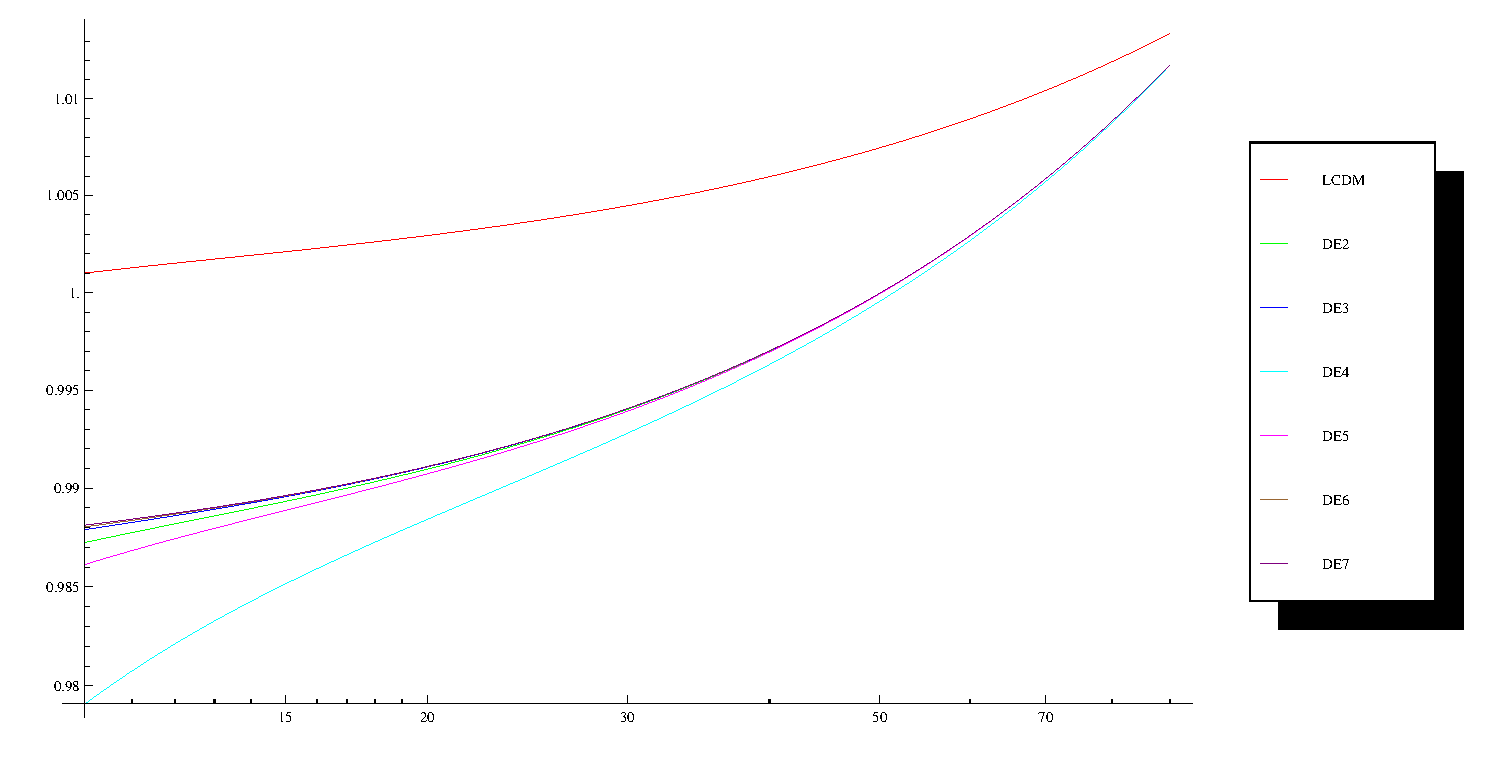
\includegraphics[width=400pt]{CPL_Sync_2012-02-20_Growth2.eps}
\caption{CPL parameteriztion. $w2$: $w20=-1$, $w2a=0.1$; $w3$: $w30=-1$, $w3a=-0.1$; $w4$: $w40=-0.92$, $w4a=0.35$; $w5$: $w50=-0.9$, $w5a=0.1$.}\label{fig:Growth2_CPL_SynchronousGauge_2012-02-19}
\end{figure}

\begin{figure}[!htbp]
\centering
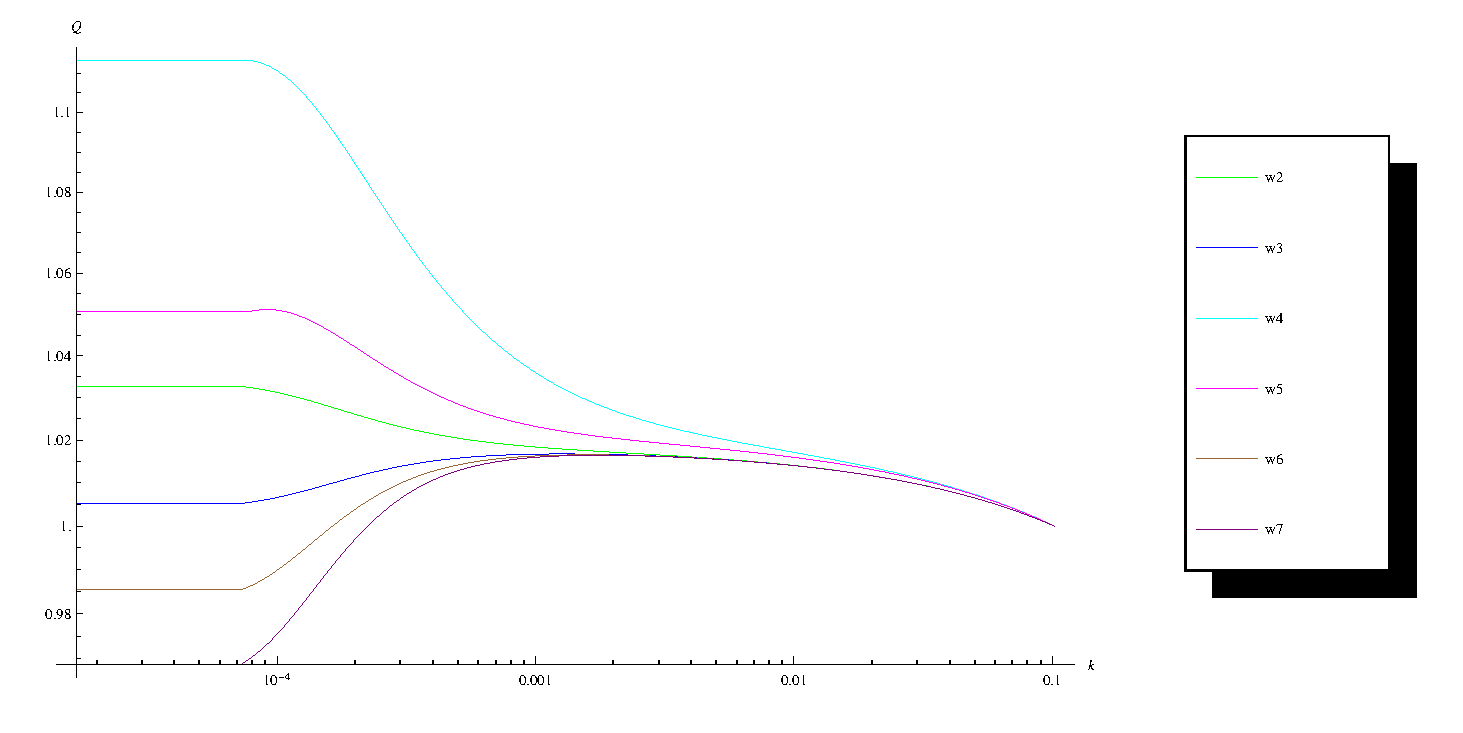
\includegraphics[width=400pt]{CPL_Sync_2012-02-20_QFactor.eps}
\caption{CPL parameteriztion. $w2$: $w20=-1$, $w2a=0.1$; $w3$: $w30=-1$, $w3a=-0.1$; $w4$: $w40=-0.92$, $w4a=0.35$; $w5$: $w50=-0.9$, $w5a=0.1$.}\label{fig:QFactor_CPL_SynchronousGauge_2012-02-19}
\end{figure}

\begin{figure}[!htbp]
\centering
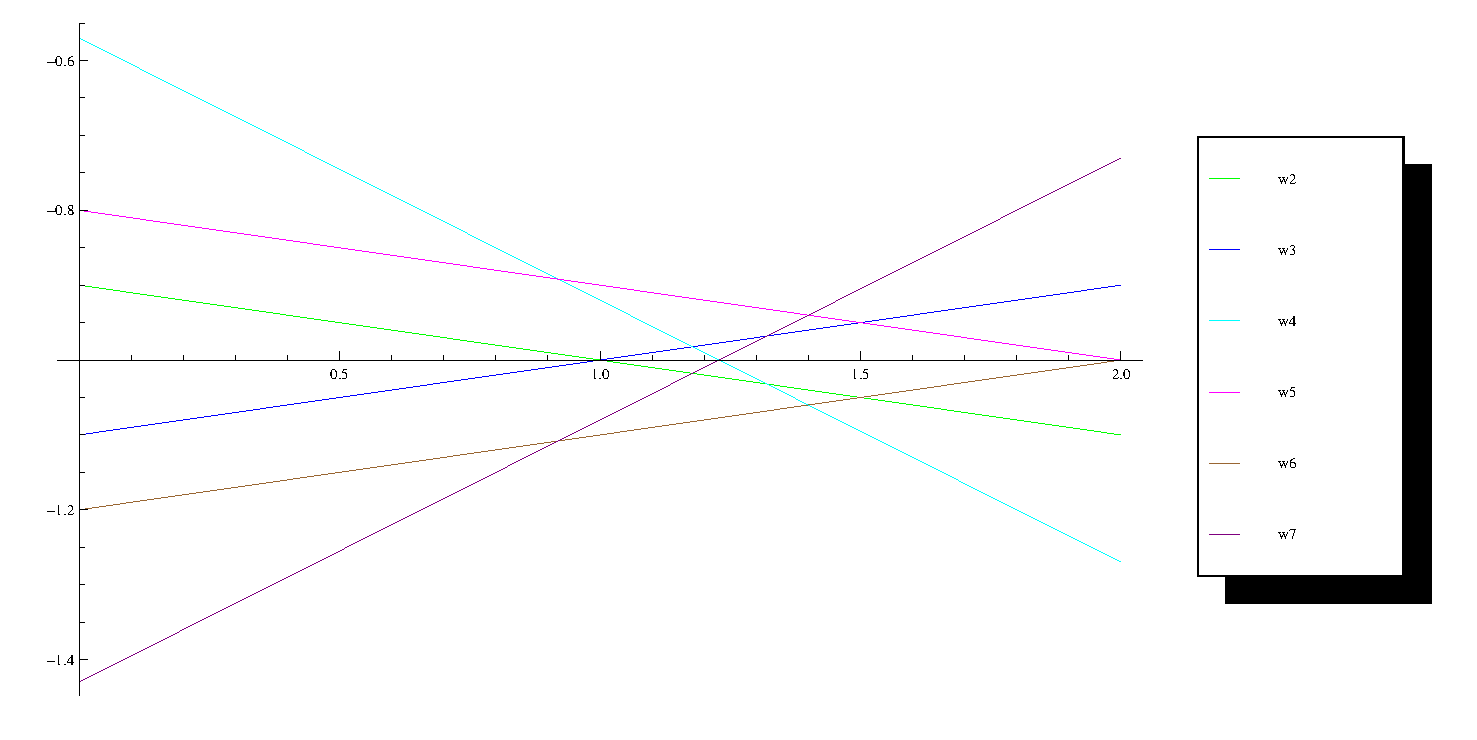
\includegraphics[width=400pt]{CPL_Sync_2012-02-20_EoS.eps}
\caption{CPL parameteriztion. $w2$: $w20=-1$, $w2a=0.1$; $w3$: $w30=-1$, $w3a=-0.1$; $w4$: $w40=-0.92$, $w4a=0.35$; $w5$: $w50=-0.9$, $w5a=0.1$.}\label{fig:EoS_CPL_Sync_2012-02-19}
\end{figure}



The parameters are mostly chosen according to the constrains of SNe Ia data and BAO data.{\footnote{arXiv:0905.1234. Also referenced arXiv:0804.0389 etc.}}


\vspace{2ex}
\hrule
\vspace{2ex}

\sout{
This is an example calculation of CPL parameterization. I'll read He's paper to find out what parameters to calculate.
}

\vspace{2ex}
\hrule
\vspace{2ex}


}

\subsection{Interaction Model}

\paragraph{Reminder:} Among the calculations, $\mathcal R \equiv \frac{1}{\mathcal H}(H_L+\frac{1}{3}H_T)\sim \frac{1}{k^2}$, so NEVER drop $k^2 \mathcal R$. Also, $V\sim \frac{1}{k}$.


\paragraph{Background}

\begin{eqnarray}
\rho_m'+3\mathcal H \rho_m =3\mathcal H (\delta_1\rho_m+\delta_2\rho_d)  \\
\rho_d'+3\mathcal H \rho_d(1+w_d)=-3\mathcal H(\delta_1\rho_m+\delta_2\rho_d)
\end{eqnarray}


\paragraph{Perturbation}:



Density equations 
\begin{eqnarray}
\delta_m'+kv_m=-3H_L'-3\delta_2\mathcal H \frac{\rho_d}{\rho_m}\delta_m+3\mathcal H\delta_2 \frac{\rho_d}{\rho_m}\delta_d    \\
\delta_d'+3\mathcal H (1-w_d)\delta_d =-(1+w_d)kv_d-3(1+w_d)H_L'
\end{eqnarray}

Velocity equations
\begin{eqnarray}
v_m'+\mathcal H (1+3\delta_2 \frac{\rho_d}{\rho_m})v_m=0 \\
v_d'+\mathcal H (1-3w_d+3\delta_2)v_d=\frac{k}{1+w_d}\delta_d
\end{eqnarray}


Define $\lambda=\rho_d/\rho_m$ and $c_{sd}^2=1$, $c_{ad}^2=w_d$.

\iffalse
\begin{eqnarray}
&&\delta_m''+\mathcal H (1+3\delta_2\lambda)\delta_m' \\
&=&-3H_L''-3H_L'\mathcal H (1+3\delta_2\lambda)+3\delta_2(\mathcal H\lambda (\delta_d-\delta_m))'+3\delta_2\mathcal H \lambda(\delta_d-\delta_m)\mathcal H(1+3\delta_2\lambda) \\
&&\delta_d''+3(1-w_d)(\mathcal H \delta_d)'+\mathcal H (1-3w_d+3\delta_2)\delta_d'+3\mathcal H^2 (1-3w_d+3\delta_2)\delta_d(1-w_d) \\
&=&-k^2\delta_d-3(1+w_d)H_L''-3(1+w_d)\mathcal H (1-3w_d+3\delta_2)H_L'
\end{eqnarray}
\fi


{\color{blue}

Finally, the perturbation equations are

\begin{eqnarray}
(a\mathcal H) \hat{\hat{\delta_d}} &=& - (2+3 Ce^2-3w-\frac{3\delta2}{w+1}+a\frac{\hat{\mathcal H}}{\mathcal H})a\mathcal H^2 \hat{\delta_d} + [-3Ce^2 a \frac{\hat{\mathcal H}}{\mathcal H} + 3(\delta 2 + w)\frac{\hat{\mathcal H}}{\mathcal H} a \\
&& - k^2 Ce^2\frac{1}{\mathcal H^2} +\frac{3}{2}(1+w)a^{-3(1+w+\delta 2)} + 3(w-Ce^2)(1-\frac{3\delta 2}{1+w})]\mathcal H \delta_d \\
\hat{\hat{\delta_m}} &=& -(\frac 2 a + \frac{\hat{\mathcal H}}{H} + \frac{6\delta2\lambda}{a})\hat{\delta_d} + \{ 3\delta 2 \lambda \frac{1}{a^2}[ (1 + 3w) + 3\delta2 (1+2\lambda) ] - 3\delta2 \lambda \frac 1 a \frac{\hat{\mathcal H}}{\mathcal H} \\
&& + \frac 1 2 \chi^2 \frac{1}{\mathcal H^2}\rho_m \} \delta_m  + \{ 3\delta2 \lambda \frac{1}{a^2}[1-3(\delta2+w)] + 3\delta2\lambda \frac 1 a \frac{\hat{\mathcal H}}{\mathcal H} + \frac1 2 \chi^2\frac{1}{\mathcal H^2}\rho_d \}\delta_d + 3\delta2\lambda\frac 1 a \hat{\delta_d}
\end{eqnarray}

In these equations, $\hat{\delta}$ stands for derivative of scale factor $a$.



\iffalse    %%%% On 2012-02-19 Mid Night%% The eqn of \delta_d was wrong.
\begin{eqnarray}
&&\delta_d''-[3\mathcal H' (w_d-1)+3\mathcal H^2 (w_d-1)(1-3\delta_2\frac{1}{1+w_d})-k^2+\frac{1}{2}\chi^2 a^2(1+w_d)\rho_d]\delta_d  \\
&=&-\mathcal H [4-3w_d-3\delta_2\frac{1}{1+w_d}]\delta_d'+\frac{1}{2}\chi^2a^2(1+w_d)\rho_m\delta_m   \\
&&\delta_m''+\mathcal H(1+6\delta_2\lambda)\delta_m' \\
&=&{3\delta_2\mathcal H^2 \lambda [(1+3w_d)+3\delta_2(1+2\lambda)]-3\delta_2\mathcal H'\lambda +\frac{1}{2}\chi^2 a^2\rho_m}\delta_m+{3\delta_2\mathcal H^2\lambda[1-3(\delta_2+w_d)]+3\delta_2\mathcal H'\lambda +\frac{1}{2}\chi^2 a^2\rho_d}\delta_d +3\delta_2\mathcal H\lambda\delta_d'
\end{eqnarray}
\fi



To solve these two equations, we need to apply some extrodinary conditions,
\begin{itemize}
\item
Adiabatic initial conditions. Only $\delta_x=\frac13\delta_c$ used here.
\item
Sound speed: $Cs^2<1$ by hand.
\end{itemize}

The parameters should be chosen carefully since many papers mentioned about the instabilities.{\footnote{HE 09, Gavda 09, Jackson 09; Bean 08}}. To be simple, I used the paramters methioned in HE arXiv:0902.0660, and only considering $\delta1=0$ situation.


}












\section{Power Spectrum}

Growth factor is independent of wave number $k$. However, applying the idea that perturbations of different wave length come in to horizon at different time, growth factor makes different contributions to different wave number. So it would be helpful to denote the growth factor as $D_+(a,k)$, which actually can be viewed as $D_+(k)$.

Using these equations, matter power spectrum reads
\begin{equation}
P(k)=\delta_i^2 \left(\frac{D_+(a,k)}{D_+(a_i,k)}\right)^2
\end{equation}

\section{Models}

Thus we can find out the power spectrum of other dark energy models as soon as we know the growth factors.

\begin{equation}
P^{(X)}(k)=P^{(L)}\left(\frac{\delta^{(X)}_i}{\delta^{(L)}_i}\right)^2 \left( \frac{D^{(X)}_+(a,k)/D^{(X)}_+(a_i,k)}{D^{(L)}_+(a,k)/D^{(L)}_+(a_i,k)}  \right)^2
\end{equation}









\section{Numerical}

\begin{quote}
\begin{itemize}
\item
Speed of light in vacuum, $c=300000\mathrm {km/s}$.
\item
Hubble constant, $H_0=100 h \mathrm{km\cdot s^{-1}\cdot Mpc^{-1}}$.
\item
Particle horizon, $dH=c\cdot a\cdot \int^a_0 \frac{1}{x^2 H(x)}\mathrm dx$.
\item
wavenumber corresponding to particle horizon, $k(a)=\frac{1}{dH(a)}$
\item
The factor to multiply to the power spectrum of LCDM,  $Q^2$, in which \begin{equation}Q=\frac{D^{(X)}_+(a,k)/D^{(X)}_+(a_i,k)}{D^{(L)}_+(a,k)/D^{(L)}_+(a_i,k)}\end{equation}

\end{itemize}
\end{quote}


\subsection{Preparation}

Find out when do a mode $k$ come into the horizon by solving equation
\begin{equation}
k(a)=\frac{1}{dH(a)}     .
\end{equation}

For a particular mode $k$, the evolution stats at,




For the part that hasn't get into horizon they don't grow, that is to say, since we only have a power spectrum of LCDM calculated with cmbeasy we have to calculate k(1).\footnote{When calculating the power spectrum of another dark energy model, one should be careful that till now, there are may modes that is still outside of horizon. So for these modes,i.e. modes with wavelength larger than the horizon, Q should be set to some constant according to the normalization.}

\begin{center}
\begin{tabular}{cc}
	Model & k(1) \\
	sCDM & $1.68\times 10^{-4}$  \\
	LCDM & $9.85\times 10^{-5}$\\
	w=-0.1 & $1.41\times 10^{-4}$  \\
	w=-0.5 & $1.07\times 10^{-4}$ \\
	w=-0.8 & $1.01\times 10^{-4}$\\
\end{tabular}
\end{center}


Those corresonds to the following elements in 2011\_11-27.dat,


\begin{center}
\begin{tabular}{cc}
	Model & k \\
	sCDM &  37   \\
	LCDM & 28\\
	w=-0.1 & 35  \\
	w=-0.5 & 30 \\
	w=-0.8 & 29\\
\end{tabular}
\end{center}


Let's review the idea now. Power spectra are initialised at the end of the inflation, then comes into the radiation era. For different dark energy models, the have the same power spectra at the end of inflation. We can assume that all different dark energy models we are considering have the same matter power evolution at radiation era because dark energy is not functioning at this early stage. That means all models here will have the same power spectra at the end of radiation era. For simplicity, it is reasonable to use matter-radiation equality as the end of radiation domination.


Then what's the power spectra today? Ivan Duran et al. argued that
\begin{quote}
"... the power spectrum at samll scales will have the same shape in both models."
\end{quote}

In my opinion, if we only consider these conditions, the power spectra won't be the same at small scales, but different at small scales, because of the relation
\[\Delta^{(X)}(k,t_0)=\left(\frac{D(t_0)}{D(t_i)}\right)^2\Delta^{(X)}(k,t_i)=\left(\frac{D(t_0)}{D(t_i)}\right)^2\Delta^{(X)}(k',t_i')\]

in which $k$ stands for some wavenumber and $t_0$ stands for some very late time like today. $k'$ and $t_i'$ is another mode.

However as they said in the paper,
\begin{quote}
"..., this assumption guarantees that the DE model will dpass the constraints inposed by the galsxy distribution on scales $\lambda<100\mathrm {Mpc}/h$ not less well than the $\Lambda$CDM model."
\end{quote}


The idea that keeps the large wavenumber part the same is just we have to pass that galaxy distribution. Then where does the freedom come from? It's the initial density perturbation say $\delta_i$ which occurs in 
\[\delta(a)=\delta_i \frac{D_+(a)}{D_+(a_i)}  .\]


Anyway, to summarize, we have to normalize the power spectra to be the same at large wavenumber, i.e., small scales like $100\mathrm{Mpc}/h$.

One important thing to be noticed is that the factor $Q$ should have the same value asymptotically in different models.


\paragraph{Growth Factors} are calculated with the equation \ref{GrowthFactorEvo2}. Initial condition for LCDM are chosen so that at matter domination ({\bf early time?}) LCDM has the same growth factor as sCDM's. Initial conditions for other models are chosen so that at early times other models are the same as LCDM.








\subsection{Power Spectra}

\paragraph{Import Power Spectra of LCDM Calculated by {\it cmbeasy}.}

The imported power spectrum is $P(k)$.

\paragraph{Transition Points}
\begin{enumerate}
\item
Use the $k(a)$ relation calculated in preparation to find the $k$ for current day, which is denoted $k_0$. Till now there are still many modes with $k>k_0$ outside of the horizon and did not come into horizon. Thus power spectrums of this size will have the same trend with the original power spectrum of LCDM calculated by {\it cmbeasy}.

For sCDM model, this transition lies between the 31-32 elements (corresponds to $k=1.128*10^{-4}$ and $k=1.202*10^{-4}$) while the last element is at $a=0.000927$ ($k=5.610$).

For LCDM, this transition happens between the 23-24 elements (corresponds to $k=6.781*10^{-5}$ and $k=7.226*10^{-5}$). And the last element is at $a=0.000737$ ($k=5.610$).

For DE2 with $w2=-0.1$, the current day lies between the 29-30 elements (corresponds to $k=9.932*10^{-5}$ and $k=1.058*10^{-4}$) while the last elemet is at $a=0.000760$ ($k=5.610$).

For DE3 with $w3=-0.5$, the current day lies between the 24-25 elements (corresponds to $k=7.226*10^{-5}$ and $k=7.701*10^{-5}$), while the last element is at $a=0.000737$ ($k=5.610$).

For DE4 with $w=-0.8$, the current day lies between the 23-24 elements (corresponds to $k=6.781*10^{-5}$ and $k=7.226*10^{-4}$) while the last element is at $a=0.000736$ ($k=5.610$).

Collect all these into a table.

\begin{center}
\begin{tabular}{ccccc}
{\bf Model}&{\bf Element No.}&{\bf $k_0$}&{\bf $a_{earliest}$}&{\bf $k_{earliest}$}\\
sCDM&31/32&$1.128*10^{-4}$/$1.202*10^{-4}$&0.000927&5.610\\
LCDM&23/24&$6.781*10^{-5}$/$7.226*10^{-5}$&0.000737&5.610 \\
$w2=-0.1$&29/30&$9.932*10^{-5}$/$1.054*10^{-4}$&0.000760&5.610 \\
$w3=-0.5$&$24/25$&$7.226*10^{-5}$/$7.701*10^{-5}$&0.000737&5.610 \\
$w4=-0.8$&23/24&$6.781*10^{-5}$/$7.226*10^{-5}$ &0.000736&5.610
\end{tabular}
\end{center}

\item
Normalization of the power spectra is at $k\sim 0.1 h\cdot \mathrm {Mpc^{-1}}$ (corresponding to $a\sim 0.003282$ or the 138th element in {\it cdm\_11-27.dat}). This is {\bf NOT} a reasonable normalization. People always do the $\sigma_8$ normalization, which is $k=0.176 h\cdot \mathrm{Mpc^{-1}}$.
It is nice to say the absolute value of power spectrum is not physical. But the normalization at $k\sim 0.1 h \cdot \mathrm {Mpc^{-1}}$ will lead to the result that power spectrum of $w=-0.1$ dark matter model and LCDM diverge large $k$ (because dark matter in $w=-0.1$ model makes the horizon growth much slower than LCDM) and it's really inconvenient to compare such power spectra. Anyway, since that is a convention, I would rather stick to that.



\end{enumerate}

\begin{quote}
{\color{red}Make sure all the ratios are calculated under the same ratio when calculating Q factors.}
\end{quote}




\section{Results}

(Figure \ref{fig:HubbleDistances-all} to figure  \ref{fig:GrowthFactor2}.)


\begin{figure}[!htbp]
\centering
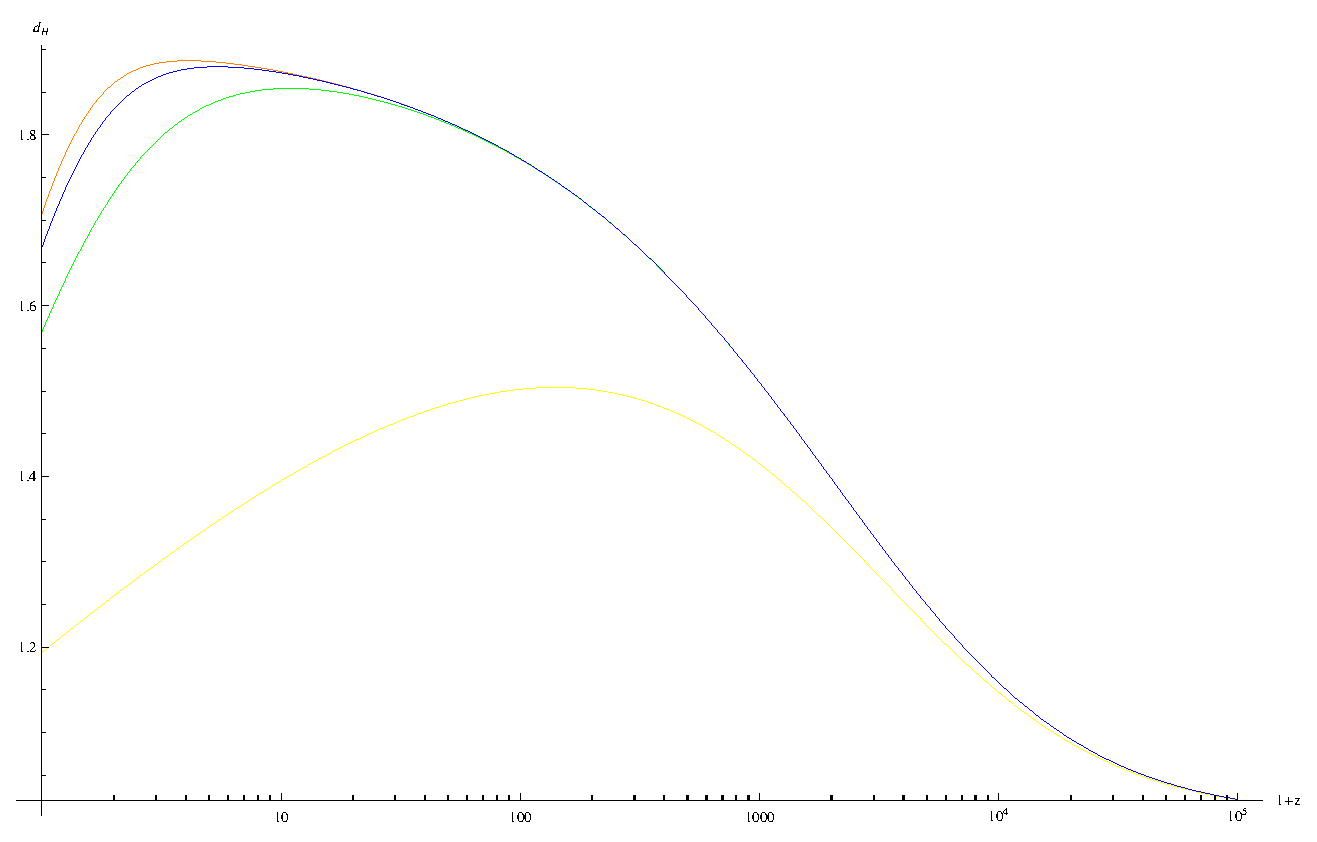
\includegraphics[width=400pt]{DEs_Sync-HubbleDistances-all.eps}
\caption{Hubble distances for all models. Orange, LCDM; Yellow, $w=-0.1$; Green, $w=-0.5$; Blue, $w=-0.8$.
Dark energy model with $w=-0.1$ has a smaller hubble distance than other models. This is the reason why the power spectrum of this model is much greater than other models: the perturbations come into the horizon much earlier.}\label{fig:HubbleDistances-all}
\end{figure}





\begin{figure}[!htbp]
\centering
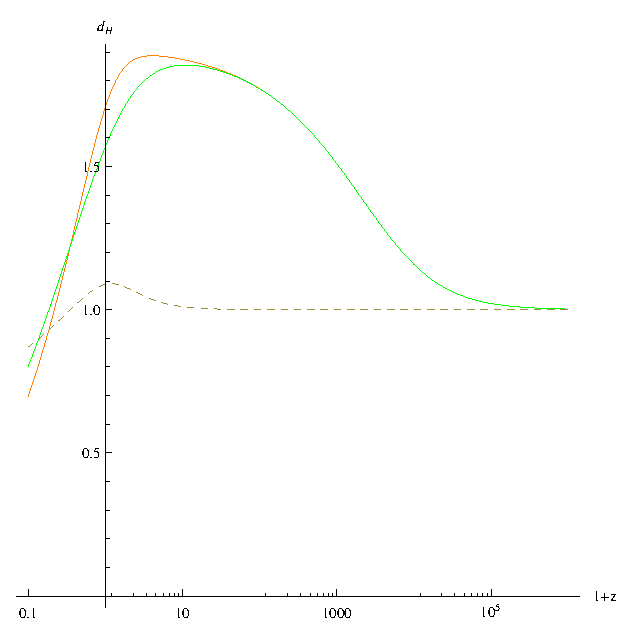
\includegraphics[width=400pt]{DEs_Sync-HubbleDistances.eps}
\caption{Hubble distances. A mimic of Ivan Duran et tal's}\label{fig:HubbleDisntances}
\end{figure}




\begin{figure}[!htbp]
\centering
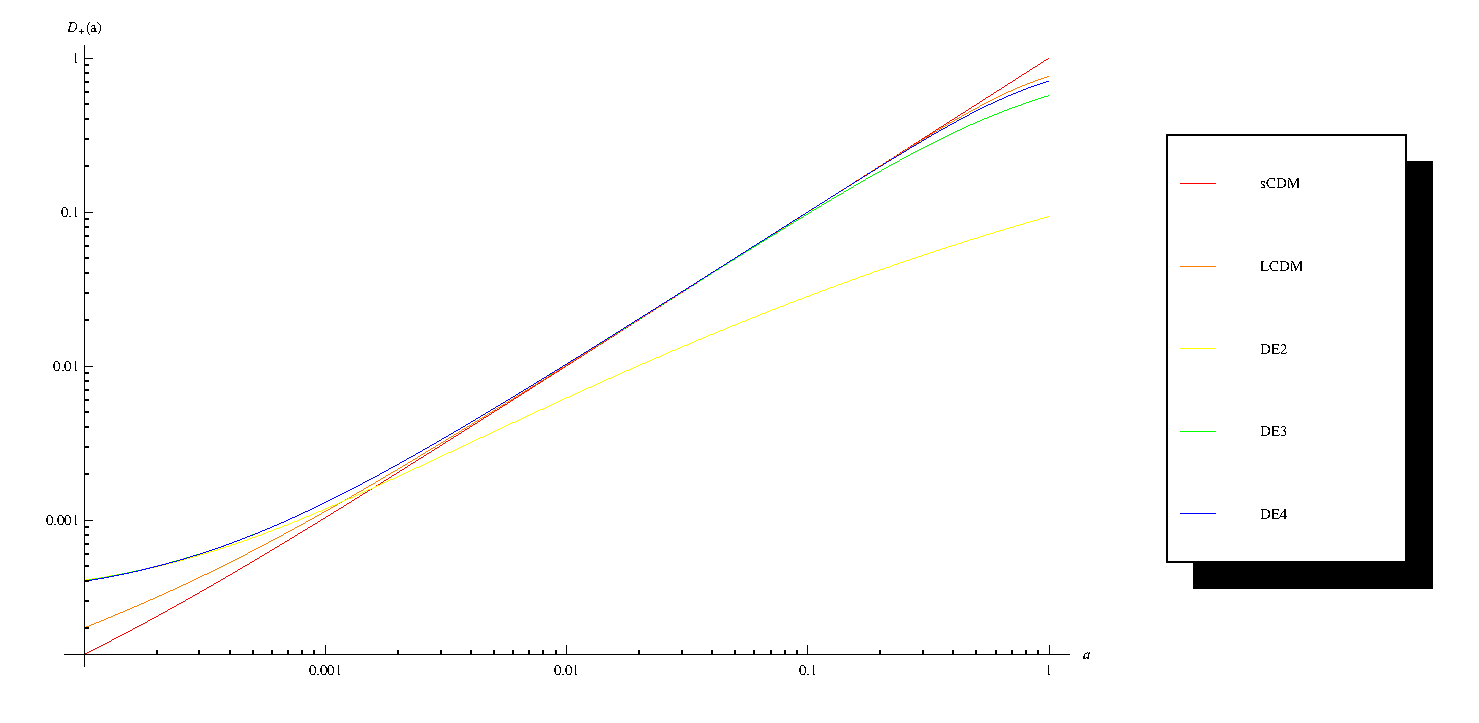
\includegraphics[width=400pt]{DEs_Sync-GrowthFactor-a.eps}
\caption{Growth factor in terms of $a$.}\label{fig:Growth-a}
\end{figure}



\begin{figure}[!htbp]
\centering
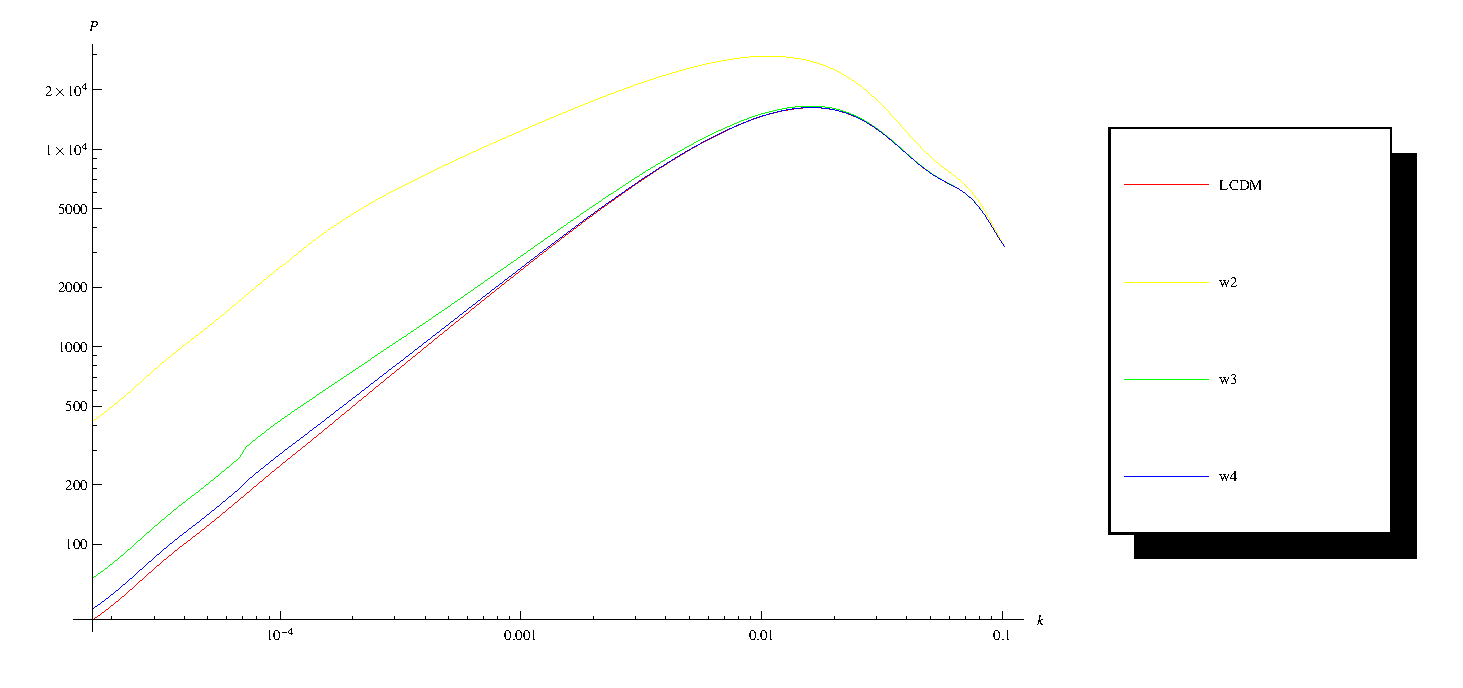
\includegraphics[width=400pt]{DEs_Sync-PowerSpectra.eps}
\caption{Power spectra}\label{fig:PowerSpectra}
\end{figure}



\begin{figure}
\centering
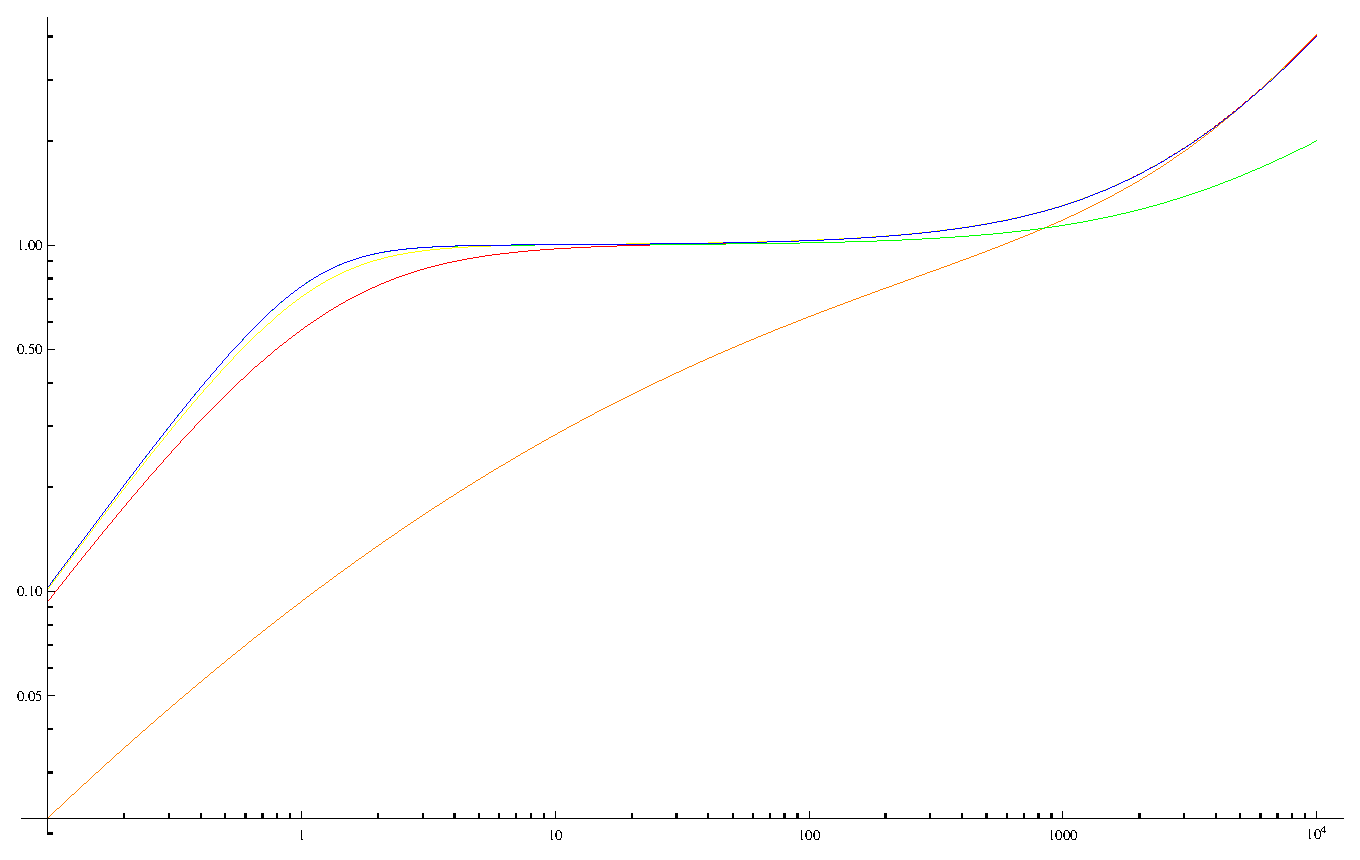
\includegraphics[width=400pt]{DEs_Sync-GrowthFactor1.eps}
\caption{Growth factor for all models. Red, $w=-0.5$;Orange, $w=-0.1$;Yellow, $w=-0.8$; Green, LCDM calculated with the approximation equation \ref{eq:GrowthFactorLCDM; Blue, LCDM calculated with the numeric solution of the original equation.}}\label{fig:GrowthFactor1}
\end{figure}

\begin{figure}[!htbp]
\centering
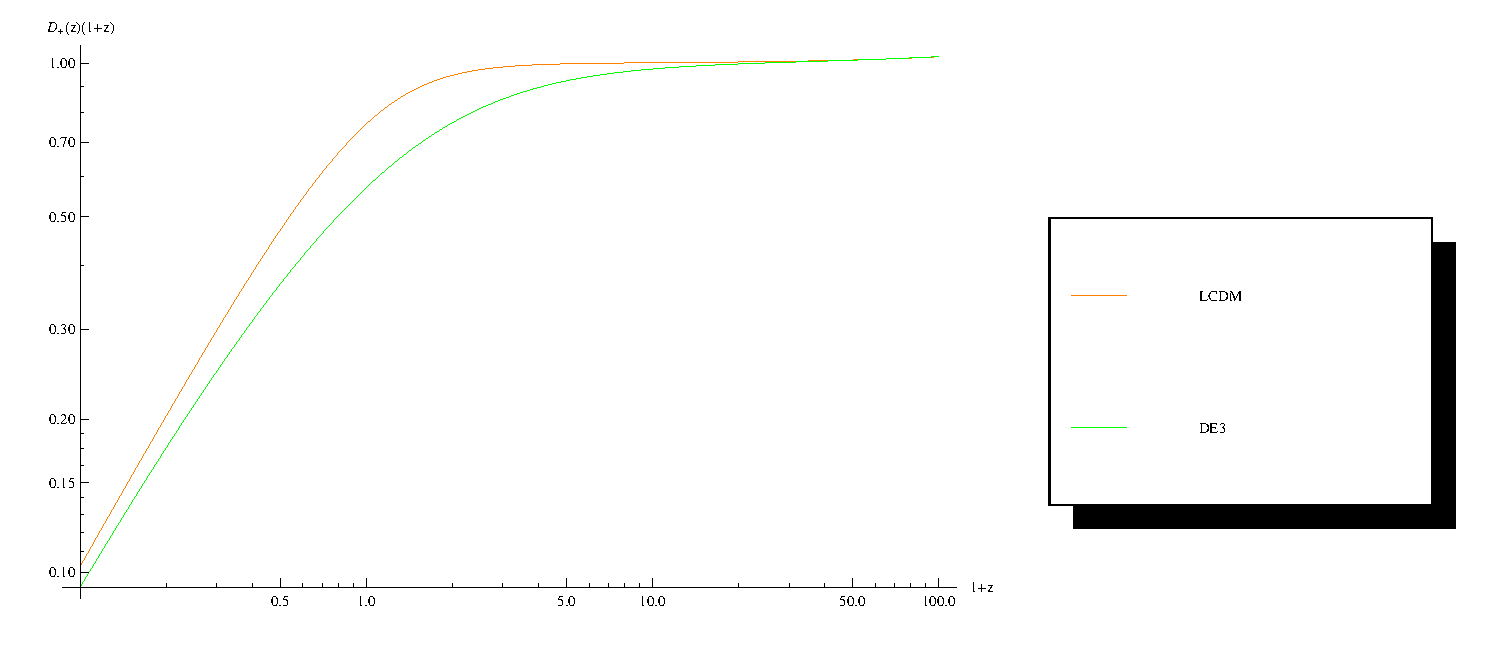
\includegraphics[width=400pt]{DEs_Sync-GrowthFactor2.eps}
\caption{Growth factor}\label{fig:GrowthFactor2}
\end{figure}



I have to mention that this calculation gives the same power spectrum as the calcution using the approximated growth factor equation. That is because dark matter starts functioning at late times and  we have cut the growth factor effect for late times because the perturbations haven't come into horizon.

As a comparison, figure \ref{fig:DEs_Sync-ApproGrowthFactor_Power} the power spectrum given by the approximated growth factor solutions.


\begin{figure}[!htbp]
\centering
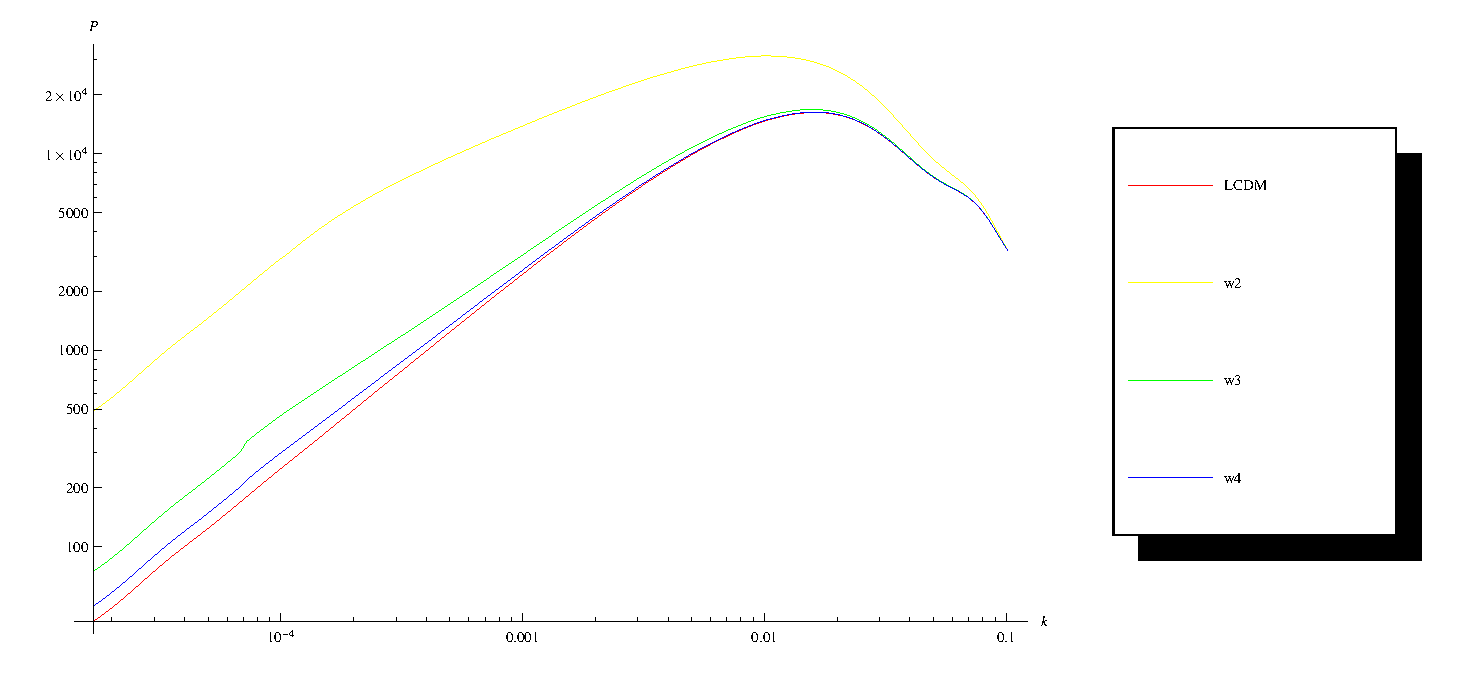
\includegraphics[width=400pt]{DEs_Sync-ApproGrowthFactor_Power.eps}
\caption{Power spectra calculated with the approximated growth factor solutions. Same as the numerical sulotion of ODE.}\label{fig:DEs_Sync-ApproGrowthFactor_Power}
\end{figure}



\section{......}

\begin{enumerate}
\item
{\sout{Equations \ref{delta1} \ref{v1} \ref{hL1} are valid under any constant EoS dark energy models.}}
\item \label{TransferFunctionQuestion}
Is it true that different models have the same transfer function for different models?

\end{enumerate}






\end{document}